\section{Workload Characterization}\label{sec:mot}

% We characterize the workload of agentic kernel optimization on top of CudaForge~\cite{cudaforge}, an efficient agentic kernel optimization system, with one generation per iteration to perform the iteration loop of \texttt{KernelBench}~\cite{kernelbench}.
We characterize the workload of agentic kernel optimization on top of the iterative refinement framework from \texttt{KernelBench}~\cite{kernelbench}, an efficient agentic kernel optimization framework for improving kernel performance.
We run two reasoning LLMs, GLM-5.1~\cite{glm5} and DeepSeek-V4-Pro~\cite{deepseekv4}, on 10 \texttt{KernelBench}~\cite{kernelbench} kernel optimization tasks widely used in LLM training and inference (Table~\ref{tab:tasks}, 100 iterations per LLM per kernel), with H200 GPUs dedicated per kernel for validation and profiling.
The resulting traces reveal three system-level inefficiencies, which we analyze in \S\ref{subsec:gen_dominates}--\S\ref{subsec:gpu_idle}.

\begin{table}[t]
    \centering
    \caption{Short names (T1--T10) of the ten \texttt{KernelBench} kernels widely adopted in LLM training and inference.}
    \vspace{-10pt}
    \label{tab:tasks}
    \small
    \setlength{\tabcolsep}{5pt}
    \renewcommand{\arraystretch}{0.90}
    \begin{tabular}{@{}llll@{}}
    \toprule
    \textbf{Abbr.} & \textbf{Task} & \textbf{Abbr.} & \textbf{Task} \\
    \midrule
    T1 & HingeLoss        & T6  & Upper-tri. Matmul \\
    T2 & 3D tensor Matmul & T7  & Lower-tri. Matmul \\
    T3 & 4D tensor Matmul & T8  & $A^{\top}B$ Matmul \\
    T4 & Diagonal Matmul  & T9  & $AB^{\top}$ Matmul \\
    T5 & Symmetric Matmul & T10 & $A^{\top}B^{\top}$ Matmul \\
    \bottomrule
    \end{tabular}
    \vspace{-10pt}
\end{table}

\begin{figure}
    \centering
    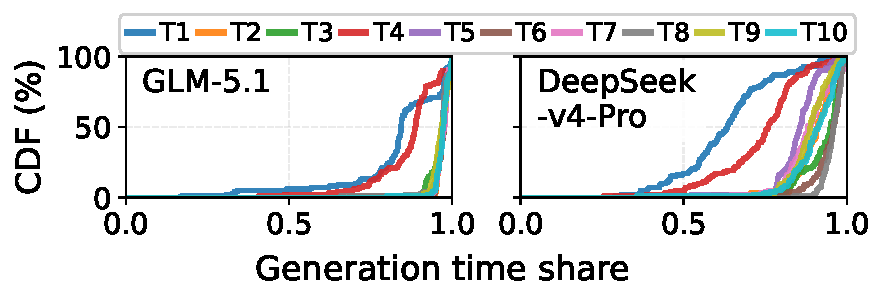
\includegraphics[width=\linewidth]{figs/generation_time_share_cdf_dual_GLM_5_1_vs_dsv4_pro.pdf}
    \vspace{-25pt}
    \caption{Per-iteration generation time share across ten \texttt{KernelBench} kernel optimization tasks per model.}
    \vspace{-15pt}
    \label{fig:generation_time_share_cdf}
\end{figure}

\subsection{Long Generation Latency}\label{subsec:gen_dominates}

We define the per-iteration \emph{generation time share} as the fraction of iteration time spent in the generation phase.
Figure~\ref{fig:generation_time_share_cdf} reports its empirical CDF across both reasoning models and the ten \texttt{KernelBench} tasks.
Under GLM-5.1, the task-level 75th-percentile (P75) of this share falls between 92--99\%, with most matmul variants clustered near 98\%. For DeepSeek-V4-Pro, P75 spans 70\%--98\%, with HingeLoss (T1) as a low outlier at 70\% and the remaining matmul workloads at P75 between 81\% and 98\%.
Across both models and the vast majority of iterations, LLM generation thus accounts for the bulk of each iteration's wall-clock, leaving validation and profiling as second-order time costs on the critical path.
In absolute terms, generation averages 706.9\,s and 522.6\,s per iteration on the two models, an order of magnitude above validation (22.9\,s and 59.0\,s) and profiling (26.5\,s and 26.6\,s).

\noindent\textbf{Reason.}
Kernel optimization is an intrinsically multi-axis problem. Each iteration must reconcile hardware constraints,
I/O and precision requirements, and evolving compute-versus-memory bottlenecks against the previous iterations' profiling
feedback. Models therefore need to reason longer to produce a kernel, leading to longer generation latency.
% \noindent\textbf{Reason.} Two factors combine to sustain this dominance consistently across the ten tasks.
% First, kernel optimization is an intrinsically multi-axis problem. Each iteration must reconcile hardware constraints,
% I/O and precision requirements, and evolving compute-versus-memory bottlenecks against the previous iterations' profiling
% feedback. Models therefore need to reason longer to produce a kernel, leading to longer generation latency.
% Second, CUDA is harder for current LLMs than popular languages. Its training corpora are far sparser than Python or general C++, and its idioms tightly couple to GPU microarchitecture (warp specialization, shared-memory bank conflicts) rather than to language-level abstractions. The model therefore spends far more tokens on CUDA kernels than on popular language code, reasoning about and emitting a full kernel source from scratch each iteration.

\noindent\textbf{Implication 1.} Long generation latency limits the iteration count under any fixed time budget, motivating a scheme to reduce the generation latency.

\begin{figure}
    \centering
    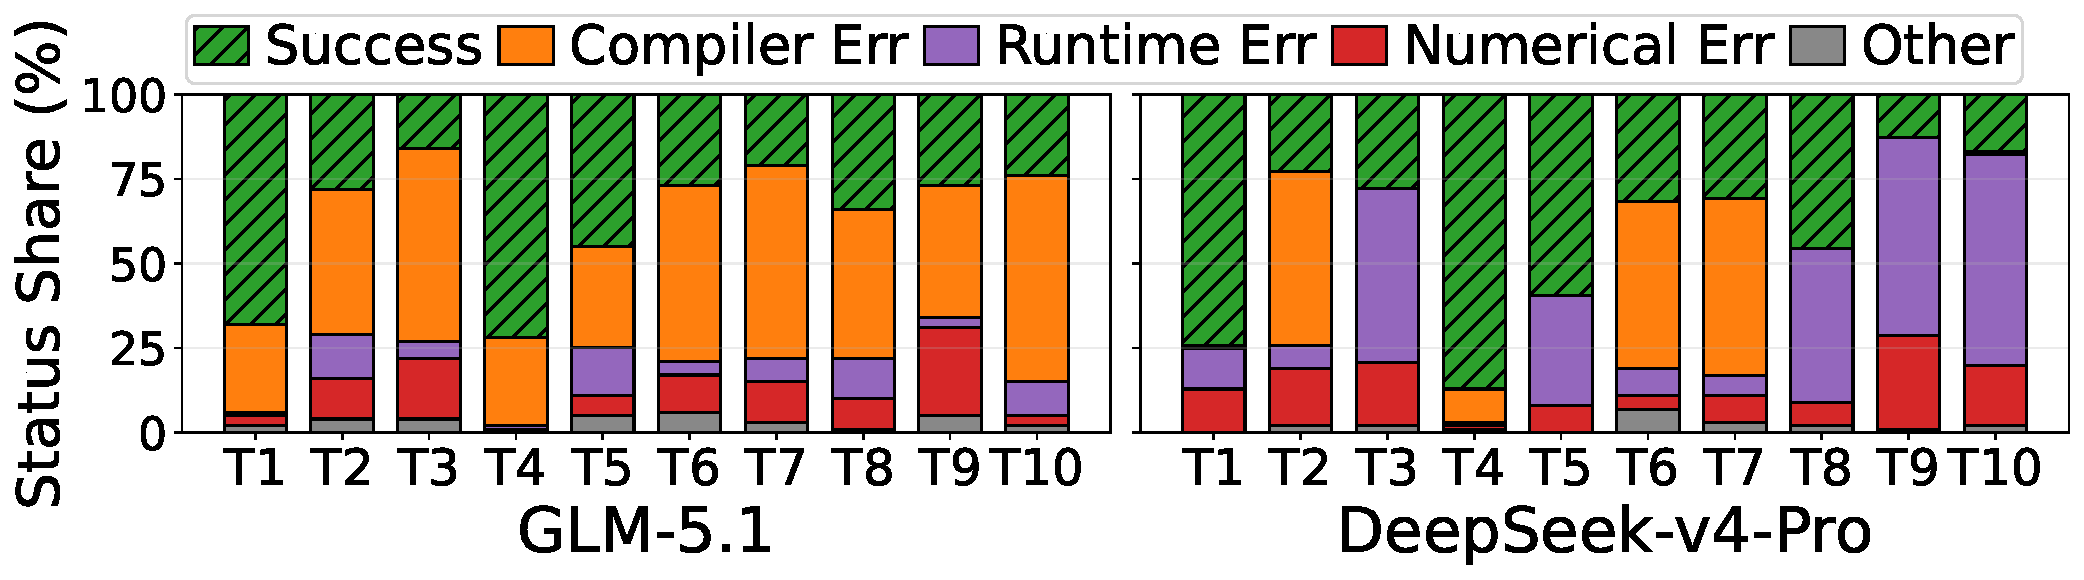
\includegraphics[width=\linewidth]{figs/task_round_outcome_ratios_dual_GLM_5_1_vs_dsv4_pro.pdf}
    \vspace{-20pt}
    \caption{Distribution of iteration status across 100 iterations per kernel with two models. An iteration is \emph{Success} iff its emitted kernel compiles, runs, and matches the reference.}
    \label{fig:iteration_status_statistics}
    \vspace{-15pt}
\end{figure}

\begin{figure*}
    \begin{subfigure}[t]{0.49\linewidth}
        \centering
        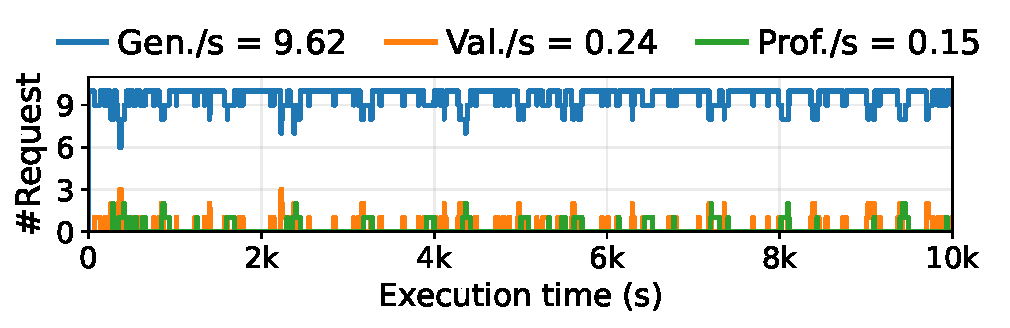
\includegraphics[width=\linewidth]{figs/phase_request_timelines_combined_GLM_5_1.pdf}
        \vspace{-20pt}
        \caption{GLM-5.1.}
        \label{fig:phase_request_timelines_GLM_5_1}
    \end{subfigure}
    \begin{subfigure}[t]{0.49\linewidth}
        \centering
        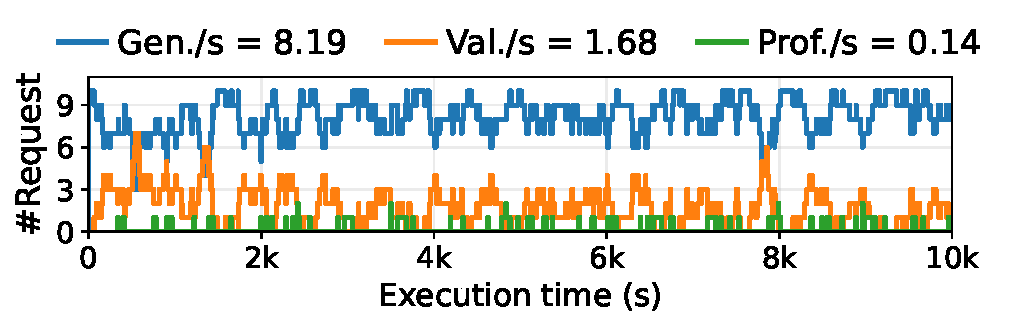
\includegraphics[width=\linewidth]{figs/phase_request_timelines_combined_dsv4_pro.pdf}
        \vspace{-20pt}
        \caption{DeepSeek-V4-Pro.}
        \label{fig:phase_request_timelines_dsv4_pro}
    \end{subfigure}
    \vspace{-10pt}
    \caption{In-flight request counts for the three pipeline phases (generation, validation, profiling) over the first 10{,}000~seconds of execution, with 10 agent workflows and 10 exclusive-mode validation/profiling GPUs.}
    \label{fig:phase_request_timelines}
    \vspace{-15pt}
\end{figure*}
\subsection{Insufficient Profiling Feedback}\label{subsec:low_feedback}

Profiling feedback refers to the NCU profiling results of a valid kernel, which the agent uses to guide the next iteration's optimization. 
However, Figure~\ref{fig:iteration_status_statistics} shows that 36.3\% of iterations under GLM-5.1 and 40.7\% under DeepSeek-V4-Pro produce kernels that pass both validation and profiling. 
On seven of the ten tasks, fewer than half the iterations yield profiling feedback.
Failure modes vary by model. GLM fails predominantly at compile time on the harder
matmul variants, indicating brittle code shape and syntax (e.g., templates, kernel signatures, includes).
DeepSeek shows more runtime failures, suggesting it compiles more aggressive variants whose indexing,
memory access, or launch configurations are unsafe. Numerical mismatches recur on transpose and
triangular matmul for both models, pointing to subtle layout or accumulator bugs that pass static checks but
produce incorrect outputs.

\begin{table}[t]
    \centering
    \scriptsize
    \setlength{\tabcolsep}{2pt}
    \caption{Best speedups over the \texttt{KernelBench} reference from 100 non-reasoning generations w/o and w/ conditioning on \emph{reasoning prefixes} with two models.
\ding{55}: no available kernels.}
    \label{tab:nonreasoning_speedups_w_wo_shared_prefix_cache}
    \vspace{-10pt}
    {
        \renewcommand{\arraystretch}{0.85}
        \resizebox{\linewidth}{!}{
            \begin{tabular}{lcccccccccc}
                \toprule
                Method & T1 & T2 & T3 & T4 & T5 & T6 & T7 & T8 & T9 & T10 \\
                \midrule
                GLM w/o      & \ding{55} & 0.44 & \ding{55} & \ding{55} & \ding{55} & \ding{55} & \ding{55} & \ding{55} & \ding{55} & 1.00 \\
                GLM w/       & 8.54 & 2.79 & 0.79 & 58.16 & 4.21 & 3.41 & 2.90 & 4.69 & 4.00 & 4.25 \\
                \midrule
                DSv4 w/o & \ding{55} & \ding{55} & \ding{55} & 57.27 & 0.36 & 0.81 & 0.35 & 0.44 & \ding{55} & 0.02 \\
                DSv4 w/  & 8.76 & 0.68 & 0.88 & 61.32 & 4.04 & 6.35 & 2.20 & 3.51 & 1.33 & 0.73 \\
                \bottomrule
            \end{tabular}
        }
    }
    \vspace{-15pt}
\end{table}
\noindent\textbf{Reason.} The insufficient profiling feedback stems from a gating effect between validation and profiling. Profiling measures real performance metrics on the GPU using NCU, and is meaningless for incorrect kernels. The agent therefore only profiles kernels that pass validation. The remaining iterations fail validation, never reaching the profiler.

% Furthermore, every faulty iteration forces the agent to spend the next iteration on repair rather than exploration, further inflating the generation cost characterized in \S\ref{subsec:gen_dominates}.

\noindent\textbf{Implication 2.} The insufficient profiling feedback forces much of the budget into failed candidates rather than
performance-improving exploration. This motivates mechanisms that increase the number of valid candidates reaching
profiling.

\subsection{Underutilized Validation/Profiling Resources}\label{subsec:gpu_idle}

Under the ``one GPU per kernel'' partitioning introduced in \S\ref{sec:bg}, the validation/profiling resource pool is severely underutilized.
Figure~\ref{fig:phase_request_timelines} shows the in-flight request counts for the three phases over the first 10{,}000 seconds of agentic kernel optimization.
We observe that the validation/profiling resource pool sustains only 0.14--1.68 concurrent requests per second on average, one to two orders of magnitude below the 8.19--9.62 concurrent generation requests over the same time window.
The resource utilization is 4.7\% on GLM and 11.3\% on DeepSeek.
The validation and profiling load is thus one to two orders of magnitude lower than generation.

\noindent\textbf{Reason.}
% First, as the generation phase occupies the bulk of the iteration time (\S\ref{subsec:gen_dominates}) the validation and profiling phases consume typically shorter time. As a result, validation and profiling resources remain idle for the majority of the iteration time;
% Second, the correctness requirement of kernel generation filters out incorrect kernels (\S\ref{subsec:low_feedback}), leaving progressively fewer requests to reach the profiling phase.
First, candidate kernels emerge only after the generation completes, so validation
GPUs remain idle during most of the generation phase.
Second, many candidates fail validation and never reach profiling, leaving
profiling GPUs with even fewer requests.

\noindent\textbf{Implication 3.} Validation and profiling GPUs sit chronically idle during the generation phase, 
leaving GPU resources underutilized. This motivates mechanisms that make candidate kernels available while reasoning
generation is still running.